\chapter{Dimensionality Reduction}
\label{sec:dimensionality_reduction}
Dimensionality Reduction is the process of reducing the number of random variables in such a way that the remaining variables effectively reproduce most of the variability of the dataset.
The reason for using such techniques is because of the \emph{curse of dimensionality} which is a phenomena that occurs in high-dimension but doesn't occur in low-dimension.\\
In machine learning problems that involve learning a "state-of-nature"(maybe an infinite distribution) from a finite number of data samples in a high-dimensional feature space with each feature having a number of possible values, an enormous amount of training data are required to ensure that there are several samples with each combination of values. With a fixed number of training samples, the predictive power reduces as the dimensionality increases, and this is known as the Hughes effect[3] or Hughes phenomenon (named after Gordon F. Hughes)\footnote{Wikipedia}\\
It happens, in general, that the intrinsic dimension is small but the data is represented by a large number of features. e.g. there may be some features across which the variance is very low and hence we can safely ignore such features reducing the dimension.\\
Dimensionality Reduction helps in visualization of high-dimensional data in 2D or 3D, data compression for efficient retrieval and storage and noise removal.
In machine learning, it is often used for feature selection and feature extraction. In this work, we have successfully used dimensionality reduction for feature selection i.e., we have selected an optimal subset of features from the given data to achieve a large improvement in accuracy.\\
Next we will discuss two of the techniques which we have used in our work and present the results obtained after applying these techniques.

\section{Principal Component Analysis(PCA)}
Principal Component Analysis(PCA) is a very famous technique for dimensionality reduction in machine learning. When given a data with $n$-dimensions/features, PCA aims to find a linear subspace of dimension $d$ lower than $n$ such that this reduced space contains most of the data points and it maintains most of the variability of the data.\\
It can be easily proved that first principal component is given by the normalized eigenvector with the largest associated eigenvalue of the sample covariance matrix $S$. A similar argument can show that the $d$ dominant eigenvectors of covariance matrix $S$ determine the first $d$ principal components. Also, the projection onto the principal subspace minimizes the squared reconstruction error,
$\sum_{i=1}^{t}\|x_i-x_i^{\widehat{}}\|^{2}$.
\RestyleAlgo{boxruled}
\LinesNumbered
\begin{algorithm}[ht]
\large
\textbf{Recover basis}: Calculate $XX^T=\sum_{i=1}^{t}x_ix_i^{T}$ and let $U=$ eigenvectors of $XX^T$ corresponding to the top $d$ eigenvalues.\\
\textbf{Encode training data}: $Y=U^TX$ where $Y$ is a $d \times t$ matrix of encodings of the original data.\\
\textbf{Reconstruct training data}: $X^{\widehat{}}=UY=UU^TX$.\\
\textbf{Encode test example}: $y=U^Tx$ where $y$ is a $d$-dimensional encoding of $x$.\\
\textbf{Reconstruct test example}: $x^{\widehat{}}=Uy=UU^Tx$.
\caption{PCA Algorithm\label{alg:pca}}
\end{algorithm}
\begin{figure}[ht!]
\centering
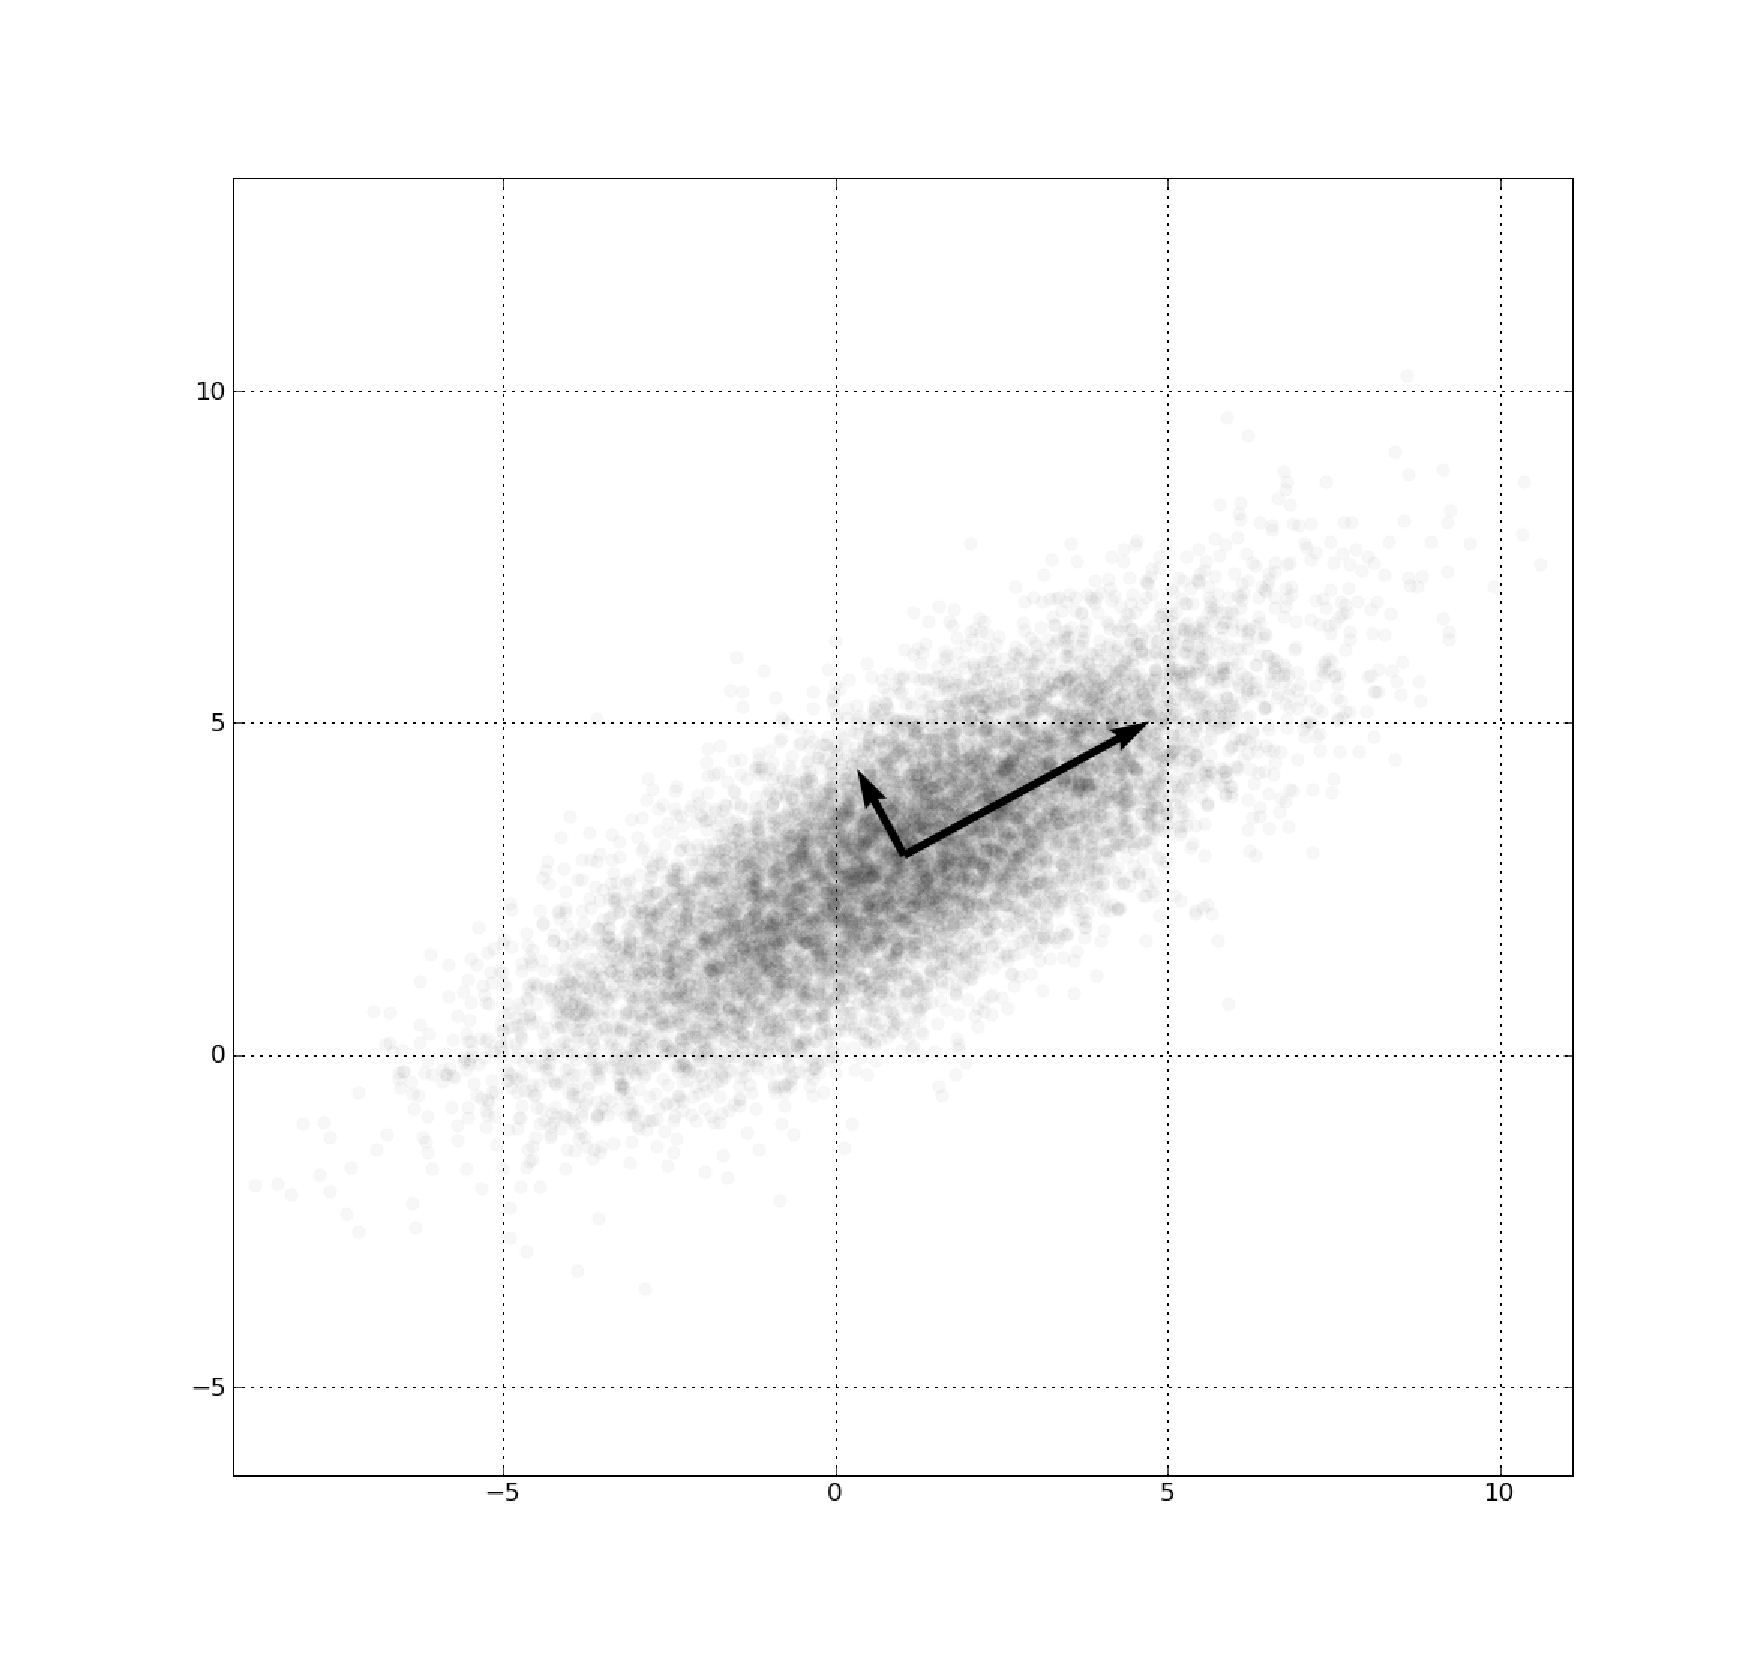
\includegraphics[width=140mm, height=120mm]{pca.eps}
\caption{PCA of a multivariate Gaussian distribution centered at (1,3) with a standard deviation of 3 in roughly the (0.878, 0.478) direction and of 1 in the orthogonal direction. The vectors shown are the eigenvectors of the covariance matrix scaled by the square root of the corresponding eigenvalue, and shifted so their tails are at the mean(Figure from \cite{wiki:2015}). \label{fig:pca}}
\end{figure}

\section{ANOVA: F-value}
Analysis of variance(ANOVA) is a set of statistical models used to analyze the differences between the group means and variation among and between groups. It was developed by R.A. Fisher. It is also a measure of statistical significance of the data point with reference to other data points present in the sample.\\
In our experiment, we have used F-test to reduce the number of features and it has led to a considerable increase in classification accuracy on our new movie dataset(Refer \ref{new_reviews}).\\
The F-statistic is calculated as:
\begin{align*}
F=\frac{\text{variance between groups}}{\text{variance within groups}}
\end{align*}
The variance between groups is given as:
\begin{align}
\frac{\sum_{i}n_i(\bar{Y_i}-\bar{Y})^2}{K-1}
\end{align}
where $\bar{Y_i}$ denotes the sample mean in the $i^{th}$ group, $n_i$ is the number of observations in the $i^{th}$ group, $\bar{Y}$ denotes the overall mean of the data, and $K$ denotes the number of groups.\\
The variance within groups is given as:
\begin{align}
\frac{\sum_{ij}(Y_{ij}-\bar{Y_i})^2}{N-K}
\end{align}
where $Y_{ij}$ is the $j^{th}$ observation in the $i^{th}$ out of $K$ groups and $N$ is the overall sample size.

\section{Result}
\begin{table}[h!]
\centering
\begin{tabular}{|c|c|c|}
\hline
\textbf{Method} & \textbf{Feature Selection} & \textbf{Accuracy} \\ \hline
\multirow{3}{*}{Document Vector}              & None      & 74.57 \\ \cline{2-3} 
                                              & PCA(n=50) & 76.33 \\ \cline{2-3} 
                                              & ANOVA-F & 88.07 \\ \hline
\multirow{3}{*}{Weighted Average Word Vector} & None      & 76.43 \\ \cline{2-3} 
                                              & ANOVA-F   & 90.37 \\ \cline{2-3} 
                                              & PCA(n=50) & 78.61 \\ \hline
\end{tabular}
\caption {Accuracies on 700-Movie Review Dataset}
\label{table:700_movie_features}
\end{table}

Table \ref{table:700_movie_features} summarizes how feature selection has improved classification accuracy on the 700 Movie review dataset. With ANOVA-F, we selected around 4k features but with PCA, this number was just 50. So, the low accuracy with PCA can be attributed to the fact that we may have lost some important features in low dimension. Also, PCA cannot work with size of dimension $d>$\emph{size of learning set}.\\
This sharp decrease in accuracy in both cases: Document vector and Weighted Average word vector happens because ANOVA-F selects features with larger variance across group and thus reduces noise to a larger extent whereas PCA reduces angular variance which is not effective in this case due to the distribution of data points in high-dimensional space.

\begin{table}[h!]
\centering
\begin{tabular}{|c|c|c|}
\hline
\textbf{Corpus} & \textbf{Feature Selection} & \textbf{Accuracy} \\ \hline
\multirow{2}{*}{Movie Reviews-IITB}   & None    & 79.17 \\ \cline{2-3} 
                                      & ANOVA-F & 89.17 \\ \hline
\multirow{2}{*}{Product Reviews-IIIT} & None    & 86.86 \\ \cline{2-3} 
                                      & ANOVA-F & 90.83 \\ \hline
\end{tabular}
\caption {Accuracies on IITB Movie Review and IIIT Product Review Dataset using Document Vectors}
\label{table:review_features}
\end{table}
Again from Table \ref{table:review_features}, we observe that ANOVA-F performs much better than PCA. Reducing dimension to 4k preserves important features whereas we are losing information once that number is reduced to 50.\\
So we easily infer that with these datasets, ANOVA-F is the feature selection method to adopt.
